\documentclass[conference]{IEEEtran}

\usepackage{cite}
\usepackage{amsmath,amssymb,amsfonts}
\usepackage{algorithmic}
\usepackage{graphicx}
\usepackage{textcomp}
\usepackage{xcolor}
\usepackage{adjustbox}

\begin{document}

\title{MoIST: Mixture of Intellectuals via Student-Teachers}

\author{
  \IEEEauthorblockN{Amy Dong}
  \IEEEauthorblockA{amydong@college.harvard.edu}
  \and
  \IEEEauthorblockN{Sammy Goldston}
  \IEEEauthorblockA{sgoldston@college.harvard.edu}
  \and
  \IEEEauthorblockN{Henry Huang}
  \IEEEauthorblockA{hhuang@college.harvard.edu}
  \and
  \IEEEauthorblockN{Nicholas Yang}
  \IEEEauthorblockA{nyang@college.harvard.edu}
}

\maketitle

\begin{abstract}
  In this work, we introduce MoIST (Mixture of Intellectuals via Student-Teachers), a novel framework that combines Knowledge Distillation (KD) and Mixture of Experts (MoE) to improve model efficiency. MoIST distills knowledge from a large teacher model into multiple smaller, specialized student models, which are then routed to handle specific subsets of the dataset. This routing mechanism, inspired by MoE, improves computational efficiency while maintaining model performance. We explore various architectural configurations for both the student models and the routing mechanism, demonstrating that MoIST can achieve accuracy comparable to the teacher model while significantly decreasing computational cost. Our results show that MoIST provides a promising approach to training an extra-efficient model, particularly in environments with limited resources.
\end{abstract}

\section{Introduction}
In recent years, significant efforts have focused on developing deep learning models that are both computationally and memory efficient, enabling their deployment on devices with limited resources. With a computational bottleneck being reached, researchers are looking to optimize aspects of machine learning algorithms so that fewer computational resources are required while running these models.

Our approach draws upon two core ideas that have reduced computation in other machine learning models: Knowledge Distillation (KD) and Mixture of Experts (MoE). In short, we take a large, pretrained teacher model and distill its knowledge to a set of smaller student models. We then employ a routing mechanism to assign and specialize each student model to a disjoint subset of the dataset. This router then selects the appropriate student model to perform inference. Instead of having a large model perform inference on a data point, that data point is routed to a smaller, specialized student tailored to that specific field, where inference is then conducted.

\section{Related Works}

\subsection{Knowledge Distillation}
Originally introduced by Hinton in \cite{hinton2015distillingknowledgeneuralnetwork}, KD resolves the large computational cost in model ensembling by distilling the ensemble into one compact model, saving computations while preserving accuracy. This is done through a combination of the soft labels that the teacher model provides and the loss that a hard label provides, transferring the teacher model's knowledge to the student model without transferring the weights. Chang et al. showed in \cite{chang-etal-2022-one} how to train multiple student models from one teacher model with KD by differentiating students by the ``views'' that they are focused on, where each ``view" corresponds to a specific feature group within the data.

\subsection{Mixture of Experts}
MoE uses a set of models, each specialized in some way, and ensembles their outputs to produce the MoE's output. This is demonstrated in Switch Transformer \cite{fedus2022switchtransformersscalingtrillion}, where Fedus, Zoph, and Shazeer show an implementation of the MoE within the feed-forward network (FFN) in the Transformer. Given a router, it determines which expert FFNs to send the data to, and outputs a weighted average of the top $k$ FFNs through a top-$k$ gate. The Switch Transformer also uses a modified loss function that considers load balancing to ensure that each expert is equitably used.

\section{Approach}

We propose MoIST: a Mixture of Intellectuals via Student-Teachers, depicted in Fig \ref{frameworkMoist}. Our model involves a combination of KD and MoE. First, we have a teacher model that distills its knowledge to multiple duplicate students. We then have a router that will divide the input dataset's class labels into subcategories. The router will then assign each student a designated subcategory, allowing them to become specialized in producing correct outputs for our model. Through this, we can create multiple smaller student models, each of which will perform comparably to the original teacher model on its assigned subset while being a fraction of the computational cost.

\begin{figure}[ht!] %!t
  \centering
  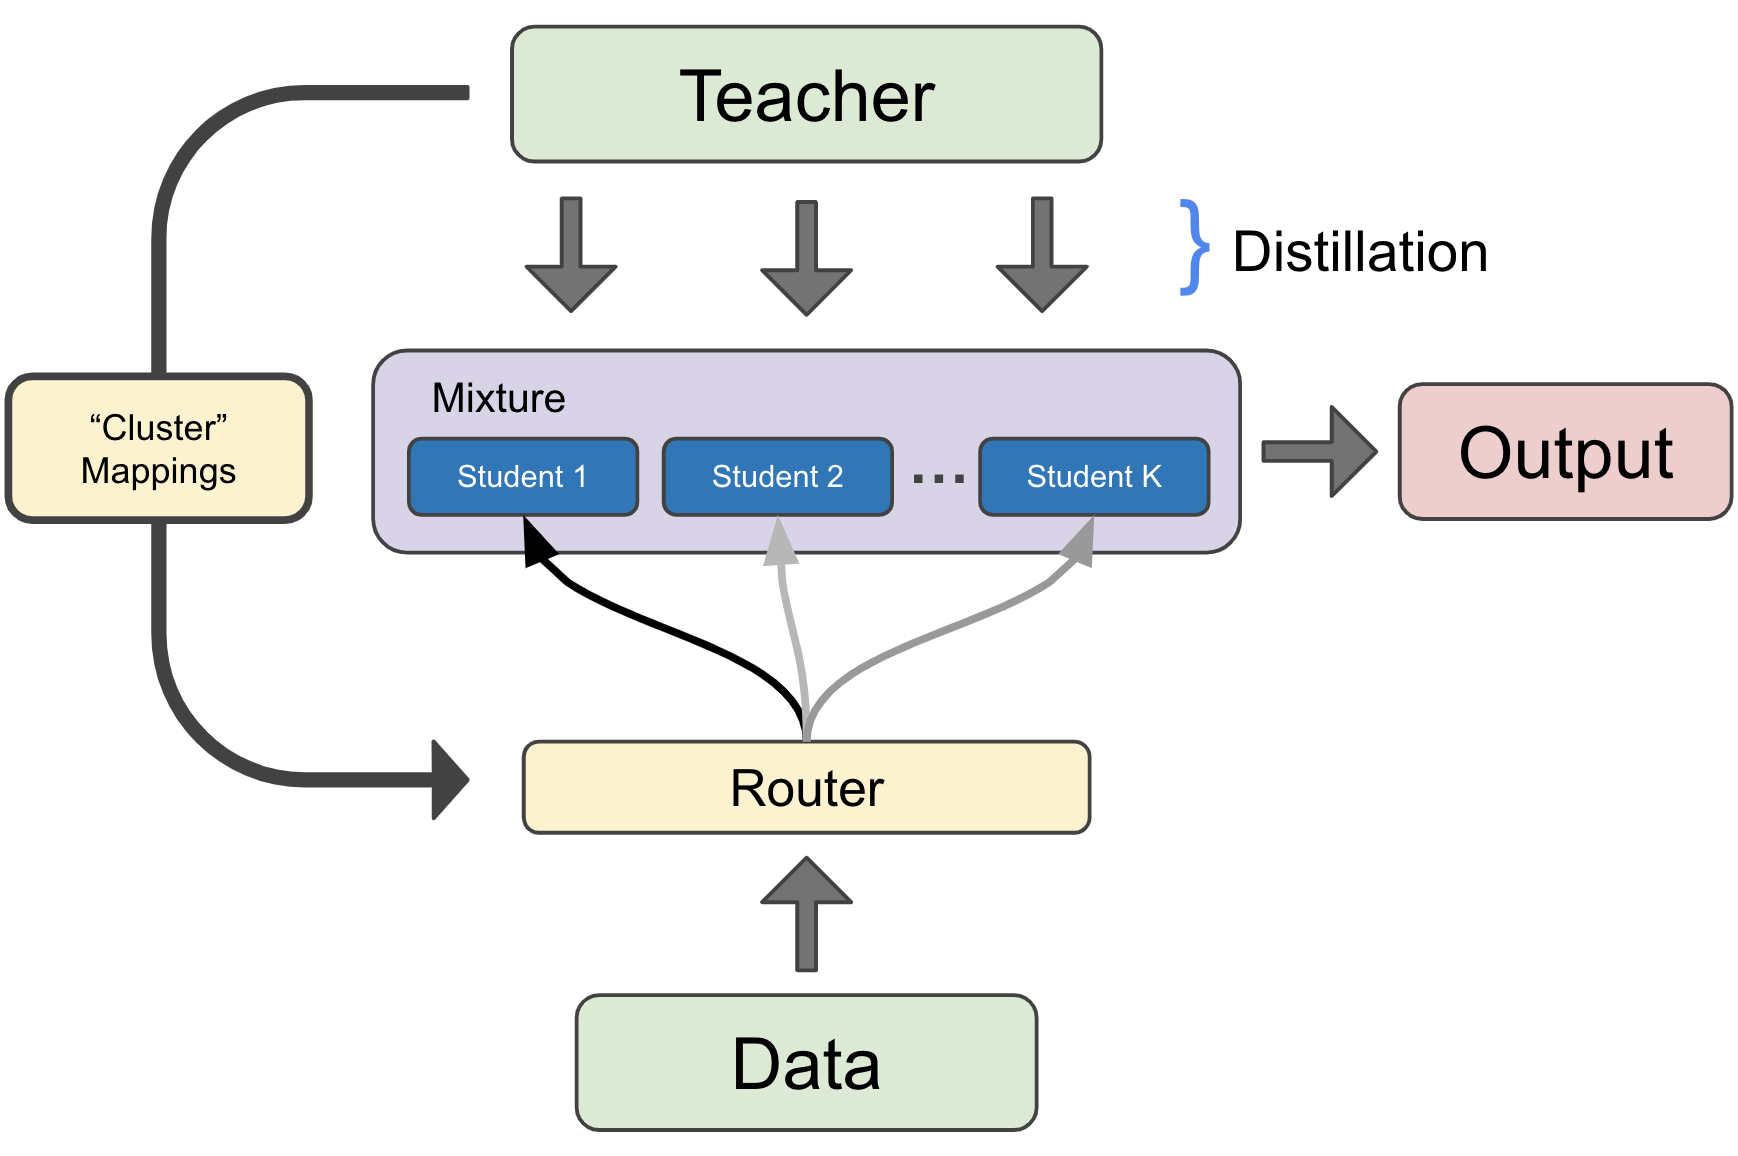
\includegraphics[width=2.5in]{figures/MoIST_framework.png}
  \caption{Framework for MoIST, combining Student-Teacher KD and MoE}
  \label{frameworkMoist}
\end{figure}

%% make a logit one, roughly draw a picture on a piece of paper

Our novel design is based on the premise of assigning students a specialized subset of data, also known as clusters. Each cluster serves as a high-level category, mapping the original labels for routing decisions, so that each student takes charge of their assigned cluster. The router is designed to be a gating network that can process the input and predict which cluster the input falls into, which then determines which student the input image is routed to for specific class label classification.

In particular, we emphasize the concept of self-partitioning rather than manual clustering of the input dataset. We achieve this by using the logits extracted from the teacher model to partition the original class labels into $k$ clusters, where $k$ corresponds to the number of students. This allows each cluster to be comprised of the most similar class labels, such that each student specializes into an expert akin to MoE principles.

Once the students have been distilled from the teacher and the router has been pretrained to classify clusters, we implement a joint training mechanism: given $k$ student models, the specialized router will train all $k$ student models by feeding them data only from their designated $k$ clusters. This allows the students to self-specialize to a subset of the dataset and have the router learn how to send different classes of input data to the corresponding student. One of the key strengths of MoIST is its avoidance of ad-hoc steps during the clustering and routing process. Every step in our framework is derived from the teacher's data learning process. MoIST ensures a data-driven, adaptable, and efficient solution.

\section{Implementation}
We utilized PyTorch, TorchVision, and FVCore for model development and performance analysis. As a proof-of-concept, a modified ResNet-18 architecture, tailored for CIFAR-10, was employed as the teacher model. Adjustments included replacing the initial convolution layer and removing the max-pooling layer to more effectively accommodate the shape of CIFAR-10 data. The teacher model was trained using cross-entropy loss with an AdamW optimizer and a learning rate scheduler to optimize convergence.

For the prototype MoIST model, simple CNNs--consisting of two convolution and two fully connected layers--were developed for the student models. KD was used to transfer the teacher's knowledge to each student, guided by a combined loss function, blending soft label loss (via KL divergence) and hard label loss (cross-entropy). To increase training efficiency, one student was distilled and its weights were duplicated to create $k$ identical students. This would allow the students to be initialized with the same knowledge from the teacher model and reduce the number of epochs necessary for convergence.

For the prototype router, we used a CNN with temperature-scaled softmax output that processes input images to predict routing probabilities for each student model. It was pretrained using hard cluster labels derived from the teacher's logits, so that the router could classify input into designated clusters assigned to each student. To create the cluster mappings using the teacher's logits, $k$-means clustering was applied to group the original CIFAR-10 classes into $k$ clusters. A cosine annealing learning rate scheduler was applied to stabilize training. Joint training of the MoIST router-student framework was conducted by combining the routing and student prediction tasks using cross-entropy loss.

The performance of the teacher model and MoIST framework was evaluated on the test dataset for accuracy and computational efficiency, measured by latency and floating-point operations (FLOPs). To explore the optimization of our model through different parameters, we performed parameter sweeps in the following categories: (1) the number of students, (2) the size of the individual students, and (3) the design of the router.

All models were trained for 20 epochs. This choice reflects the exploratory nature of our work and the preliminary stage of this analysis. While additional training epochs could potentially improve the performance of both the teacher model and MoIST, 20 epochs represented a balanced approach given our computational resources. Future work will explore extending the training duration to further refine and validate the model's effectiveness in a more resource-intensive setting.

\section{Results}

Our results are summarized in Table \ref{table:performance_comparison} and details are provided in the following sections.

\subsection{Baseline Comparisons}

To ensure that all runs are comparable, we trained one CIFAR-10-adjusted ResNet-18 teacher model for 20 epochs, achieving a test accuracy of 83.80\% and a loss of 0.4910. The teacher model achieved a latency of 6.511 ms and used 8.70 MFLOPs of computation.

We also distilled and pretrained one CNN student model for 20 epochs from the above model, which achieved a test accuracy of 79.35\% and a loss of 0.6332. The student model achieved a latency of 6.591 ms and used 0.10 MFLOPs of computation.

\subsection{Proof-of-Concept MoIST}

We implemented a proof-of-concept of MoIST to prove that specializing students can improve model accuracy. We accomplish this by implementing a router that is hardcoded to provide 100\% classification accuracy for sending an assigned cluster to each student. This approach simplifies routing by directly assigning cluster-specific inputs to its assigned student without requiring a separate gating network, guaranteeing ``100\% routing accuracy.'' Four lightweight CNN students were used. The hardcoded MoIST trained the joint student-router framework for 20 epochs.

The hardcoded MoIST framework achieved a test accuracy of 89.49\%, and a loss of 0.3052. The hardcoded MoIST framework also achieved a latency of 0.534 ms and used 0.10 MFLOPs of computation, demonstrating better performance in both computational efficiency and accuracy over the original teacher model and its constituent student models.

\subsection{Prototype MoIST}

We then implemented the prototype MoIST model, trained for 20 epochs from our teacher model. We pretrained a CNN architecture router for 20 epochs on input-cluster labels, which yielded an 88.50\% routing accuracy for cluster classifications. Joint training with students yielded the following class distributions across students in the test set, as displayed in Fig \ref{routerdist}, indicating that the cluster assignments yielded promising student specialization results.

\begin{figure}[ht!] %!t
  \centering
  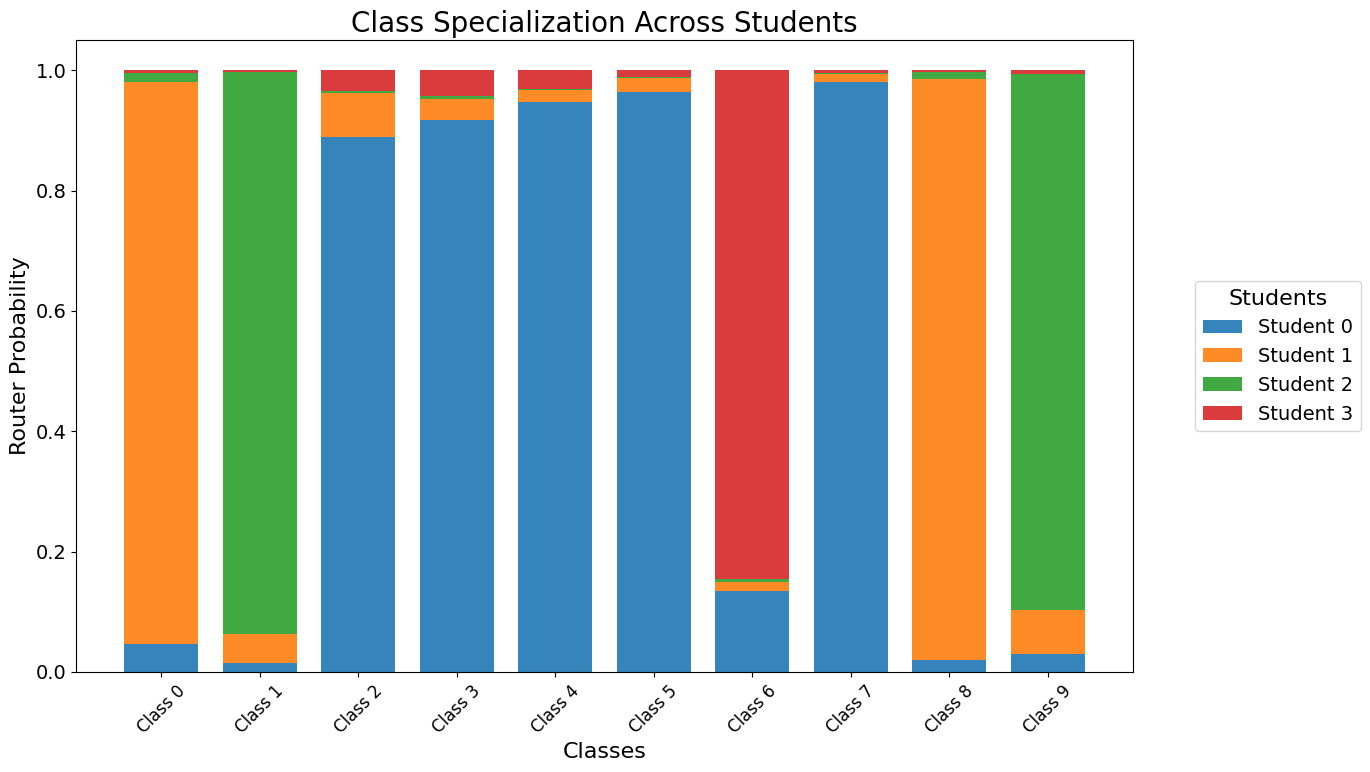
\includegraphics[width=3in]{figures/router_specialization_baseline.png}
  \caption{Prototype MoIST class specializations across students, using an 88\% accurate clustering router}
  \label{routerdist}
\end{figure}

Our prototype MoIST model achieved a test accuracy of 84.08\%, and a loss of 0.5098. In addition, it achieved a latency of 0.635 ms and used 0.10 MFLOPs of computation. Though not as over-performing as a theoretical 100\% router in accuracy, our prototype MoIST demonstrates accuracy comparable to the original teacher model. The model demonstrates a 10x improvement in latency and an 87x reduction in MFLOPs, a significant improvement in computational efficiency over the original teacher model.

\subsection{Parameter Sweeps}

\begin{table}[!t]
  \renewcommand{\arraystretch}{1.1}
  \centering
  \caption{Performance comparison of MoIST models}
  \label{table:performance_comparison}
  \begin{adjustbox}{width=0.425\textwidth}
    \small
    \begin{tabular}{|c|c|c|c|c|}
      \hline
                                               & \textbf{Accuracy} & \textbf{Loss} & \textbf{Latency (ms)} & \textbf{MFLOPs/Img} \\ \hline
      \textbf{ResNet-18 Teacher}               & 83.80\%           & 0.4910        & 6.511                 & 8.70                \\ \hline
      \textbf{Distilled Student}               & 79.35\%           & 0.6332        & 6.591                 & 0.10                \\ \hline
      \textbf{Conceptual 100\% Router}         & 89.49\%           & 0.3052        & 0.534                 & 0.10                \\ \hline
      \textbf{Prototype MoIST with CNN Router} & 84.08\%           & 0.5098        & 0.635                 & 0.10                \\ \hline
      \textbf{MoIST + Transformer Router}      & 84.01\%           & 0.5002        & 1.188                 & 0.10                \\ \hline
      \textbf{MoIST + Linear 3NN Router}       & 83.52\%           & 0.5071        & 0.945                 & 0.10                \\ \hline
    \end{tabular}
  \end{adjustbox}
\end{table}

\begin{figure}[ht!] %!t
  \centering
  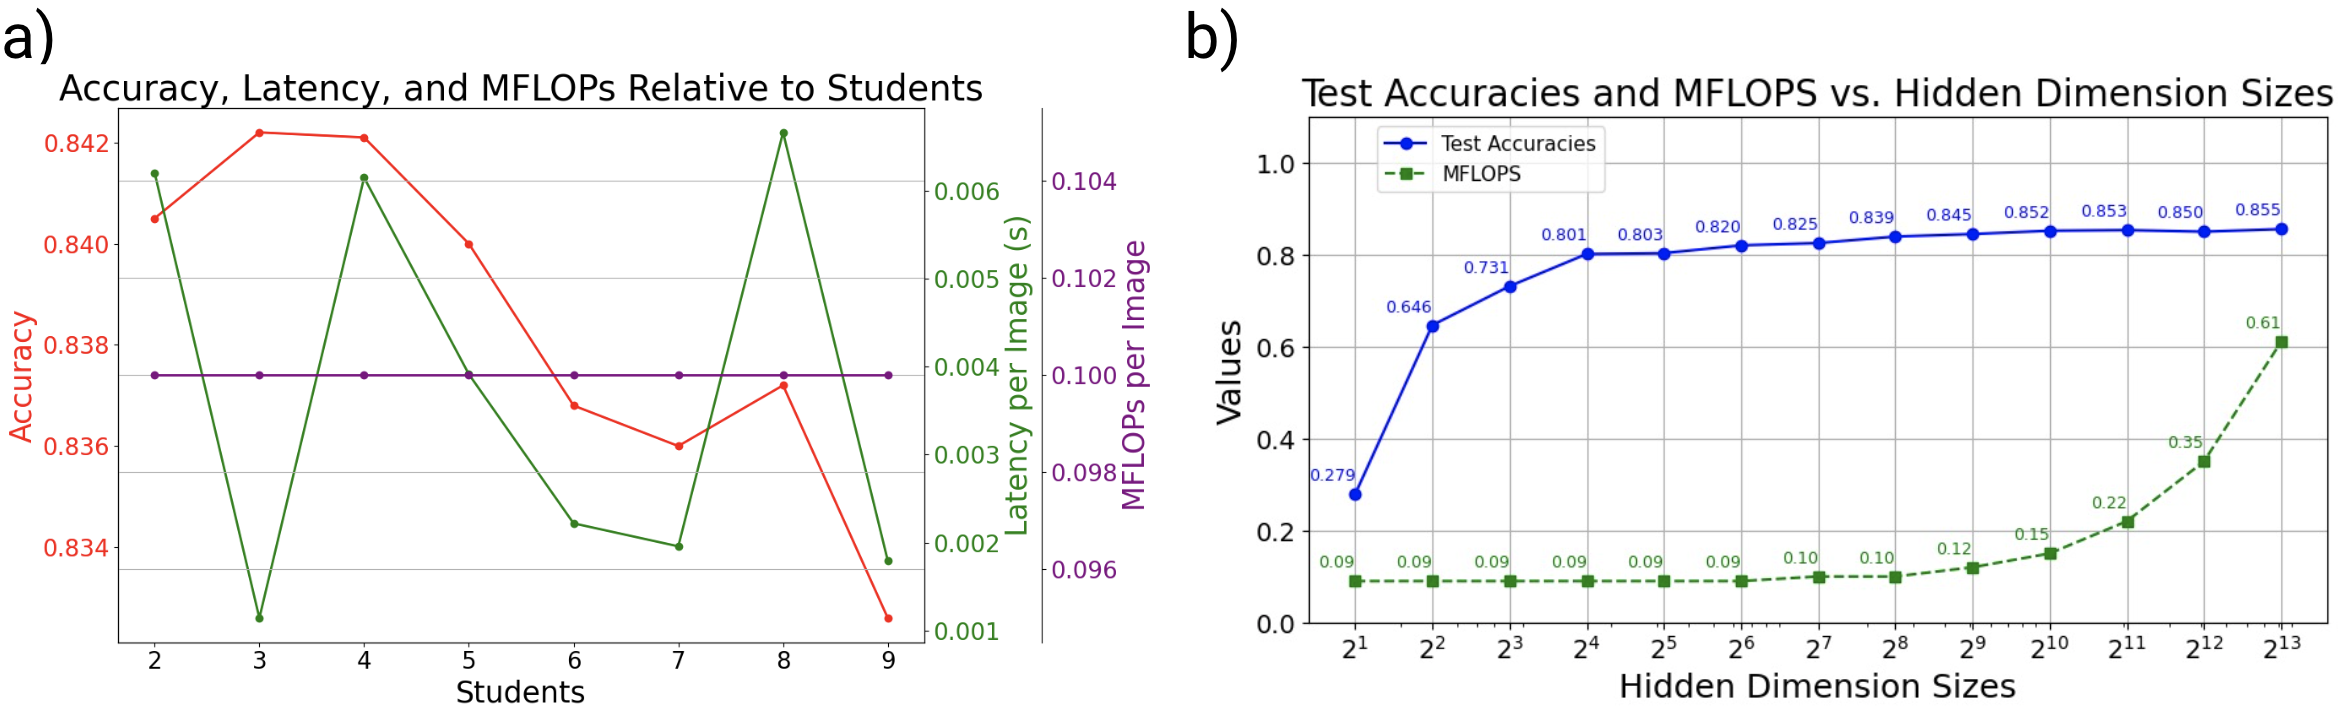
\includegraphics[width=3.45in]{figures/param_sweeps.png}
  \caption{Parameter sweeps of the prototype MoIST framework, displaying: (a) test accuracy, latency, and MFLOPs/image performance relative to the number of students employed, and (b) test accuracy and MFLOPs/image performance relative to the size of student's hidden dimension layers}
  \label{param_sweep}
\end{figure}

The objective of our parameter sweeps is to investigate the optimal MoIST architecture. Initially, we conducted a parameter sweep on the number of students, and our results indicate that a MoIST model with three students yields the highest test accuracy and the lowest latency, as illustrated in Fig. \ref{param_sweep}a. In the context of the CIFAR-10 dataset, we see that this distribution will result in all of the non-land vehicles in one cluster, on-land vehicles in one cluster, and all animals in one cluster, creating effective clusters for the students to specialize on. In the future, we plan to explore determining the optimal value of $k$ using the $k$-means clustering algorithm, rather than predefining the number of students.

Next, for the MoIST model with three students, we performed a parameter sweep on the size of the student models, specifically varying the hidden dimension width, as shown in Fig. \ref{param_sweep}b. As expected, increasing the hidden dimension size leads to an improvement in accuracy, which converges to approximately 0.85. At the same time, the MFLOPs begin at a consistent value of around 0.9 and increase exponentially once the hidden dimension exceeds $2^{10}$. Based on these observations, we conclude that the optimal balance between model performance and size occurs when the hidden dimension of the student model is approximately $2^{10}$. Notably, this optimal configuration outperforms the teacher model by 1.4\%, while requiring 58 times fewer MFLOPs.

Finally, we evaluated the router architecture using a CNN, a 3-layer linear neural network, and a transformer (2 encoder layers, 4 attention heads per layer, the input/output hidden feature vector dimensions as 64, and the dimensionality of the feedforward sublayer as 256). While all architectures performed similarly in accuracy, loss, and MFLOPs per image, we found that the prototype MoIST with CNN Router had the highest accuracy while having substantially lower latency. Additionally, we conducted a parameter sweep on the size of the Linear 3NN router and found no significant correlation between the router size and accuracy.

\section{Conclusion}

Our MoIST model maintained the same accuracy as the original ResNet-18 model that we trained and both reduced the number of computations required and inference time. While the initial proof-of-concept with manually defined data partitioning was straightforward, the development of a self-specializing router posed a larger challenge. To address this, we leveraged a clustering algorithm to guide the router's decision-making process, effectively partitioning the dataset and assigning specialized tasks to each student model. This approach not only ensured efficient routing but also demonstrated the adaptability and scalability of MoIST. Future work includes refining the routing mechanism for better generalization across different datasets and extending the training duration to improve model performance. Additionally, integrating MoIST with other model compression techniques could enhance its efficiency, making it even more suitable for resource-constrained environments.

\section{Member Contributions}
We use each team member's initials: Amy Dong (AD), Henry Huang (HH), Sammy Goldston (SG), and Nicholas Yang (NY). \textit{Project Ideation:} AD, NY; \textit{Prototype MoIST Implementation:} AD, HH, SG; \textit{Router Exploration:} SG, HH, AD; \textit{Logit-Mapping Distribution:} AD; \textit{Baseline Model Comparisons:} NY; \textit{Parameter Sweeps:} NY, HH, SG, AD; \textit{Manual Fine-Tuning Implementation:} HH, AD; \textit{Cluster Mapping Implementation:} AD; \textit{README and Documentation:} NY, HH; \textit{Paper and Slides:} AD, NY, HH.

\bibliographystyle{IEEEtran}
\bibliography{refs}

\end{document}
